\chapter{Magnetic Forces and Fields} \label{chap:MagneticForcesandFields}
	\section{Introduction to Magnetism} \index{Magnetism}
		All magnetic fields are created by moving electrically charged particles.  Since all atoms contain protons that can rotate or oscillate, as well as electrons that can move around outside the nucleus, all atoms have magnetic fields.  Most of the time, the effects of many atoms cancel out due to their random orientations.  However, sometimes atoms in areas can align, creating permanent magnetic properties in an object. 

	\section{Types of Magnetism} 
		\subsection{Permanent Magnetism}
		Permanent magnetism occurs when an object exhibits magnetic properties without any external voltages or currents being applied.  There are three basic types of permanent magnetism: 
			\subsubsection{Ferromagnetism} \index{Ferromagnetism} Ferromagnetism is the type of magnetism most of us are familiar with.  It occurs in iron, nickle, cobalt, and some types of rare-earth metals, such as neodymium.  Ferromagnetic materials are strongly attracted to external magnetic fields.  In addition, ferromagnetic materials become magnetized themselves when exposed to an external magnetic field.  That magnetization can remain even when the external magnetic field is removed.  
			
			
			\subsubsection{Paramagnetism} \index{Paramagnetism} Paramagnetic materials are weakly attracted to magnets, but do not become magnetized themselves.  Examples of paramagnetic materials include aluminum, tungsten, and platinum.  

			\subsubsection{Dimagnetism} \index{Diamagnetism} Diamagnetic materials have a weak and opposite response to magnetic fields, meaning they are repelled by a magnet. Examples of diamagnetic materials include copper, silver, and gold.
			
			
		\subsection{Electromagnetism}
		A \gls{electromagnet} is a type of magnet that is created when current flows in a wire.  Normally, an electromagnet consists of a wire that is wrapped around core made from a ferromagnetic material, such as iron.  However, all current-carrying wires - regardless of their shape - generate magnetic fields. 
		
	\section{Magnetic Force on a Charged Particle}
	
	When a charged particle moves through a magnetic field, the particle will experience a magnetic force.  That force is given by the following equation:
	
	\index{Magnetic Force on a Particle}
	
	\begin{mdframed}[backgroundcolor=orange!20!white]
		\begin{equation}
			\overrightarrow{F_B} = q \vec{v} \times \vec{B}
			\label{eqn:magforceparticle}
		\end{equation}
	\end{mdframed}
	where $\overrightarrow{F_b}$ is the magnetic force, $q$ is the charge of the particle, $\vec{v}$ is the velocity, and $\vec{B}$ is the magnetic field.  It is also important to note that the multiplication of the two vectors is a \gls{crossproduct}.
	
	Because of the cross product, a particle moving in a magnetic field always experiences a force that is perpendicular to both the magnetic field and the direction of travel.  This means that a particle could move along the following paths in a magnetic field:
	\begin{itemize}
		\item A circle $\longrightarrow$ if the magnetic field and the velocity are perpendicular.
		\item A straight line $\longrightarrow$ if the magnetic field and velocity are parallel or anti-parallel. 
		\item A helix $\longrightarrow$ if the magnetic field and the velocity are at any other angles.  
	\end{itemize}
	
		
	\begin{mdframed}[backgroundcolor=blue!10!white]
		\begin{center}
			
			
			\textbf{Example \thesection.1}	
		\end{center}
		
		\textbf{Problem: } A proton travels to the right at a speed of 256 m/s. in a magnetic field of 0.3 Teslas that is directed into the page.
		
		  \begin{enumerate}[label=(\alph*)]
			\item What is the force that the magnetic field exerts on the proton?
			\item What is the radius of the circle the proton makes?
		\end{enumerate}
		
		\textbf{Solution:} 
		\begin{enumerate}[label=(\alph*)]
		\item Begin by drawing a diagram:
		\vspace{0.1in}
		\begin{center}
			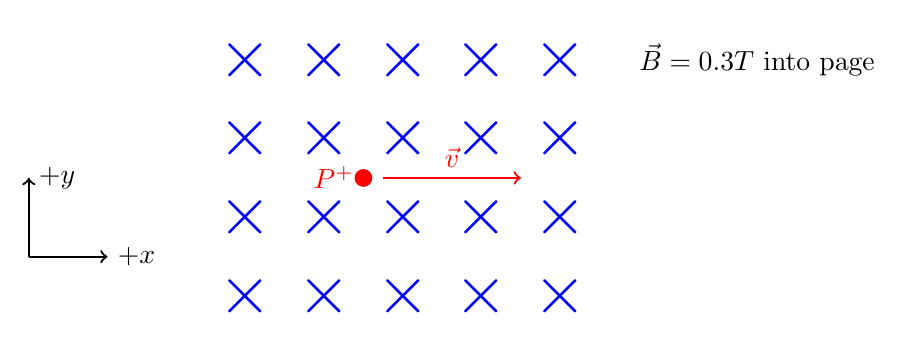
\begin{tikzpicture}
				
				% Magnetic field into the page: Xs
				\foreach \x in {0.5,1.5,2.5,3.5,4.5}
				\foreach \y in {0.5,1.5,2.5,3.5}
				\draw[thick,blue] (\x,\y) node {\Huge $\times$};
				
				% Proton
				\filldraw[red] (2,2) circle (3pt);
				\node[left,red] at (2,2) {$P^+$};
				
				% Velocity vector (right)
				\draw[->,thick,red] (2.25,2) -- ++(1.75,0) node[midway,above] {$\vec{v}$};
				
				% Magnetic field label
				\node at (7,3.5) {$\vec{B} = \SI{0.3}{T}$ into page};
			
				\draw[->,thick] (-2.25,1) -- ++(1,0) node[right] {$+x$};
				\draw[->,thick] (-2.25,1) -- ++(0,1) node[right] {$+y$};
			\end{tikzpicture}
			
		\end{center}
		
		The force on the particle is given by equation \ref{eqn:magforceparticle}:
			\begin{equation*}
			\overrightarrow{F_B} = q \vec{v} \times \vec{B}
		\end{equation*}
		
		
	 We begin by applying the first right hand rule (see \cref{RHR1}).  
	  \eqref{eqn:kineticenergy} to solve the problem.  Using the First Right Hand Rule, we find that the direction of the force on the proton is toward the top of the page.  
	  
	  Solving for the magnitude of the force, we find:
	  
	  	\begin{equation*}
	  	|\overrightarrow{F_B}| = |{q \vec{v} \times \vec{B}}| = qvB \sin(\theta) = (\SI{1.6E-19}{C})(\SI{256}{m/s})(\SI{0.3}{T}) \sin(90 \degree) 
	  \end{equation*}
  	\begin{equation*}
  	|\overrightarrow{F_B}| \approx \boxed{\SI{1.229E-17}{N}}
  	\end{equation*}
	
		\item To find the radius of the circle the particle goes in, we recognize that the magnetic field is acting as a centripetal force.  Recalling equation \ref{equation:centripetalforce}:
		
		\begin{equation*}
			F_c = \frac{mv^2}{r}
		\end{equation*}
		
		
		we can write the following equations to derive the radius of the circle:
			
		\begin{equation*}
			F_B = F_c
		\end{equation*}
		\begin{equation*}
			 qvB \sin(\theta) = \frac{mv^2}{r} 
		\end{equation*}
		\begin{equation*}
			r = \frac{mv^2}{qvB \sin(\theta)}
		\end{equation*}
	\begin{equation*}
		r = \frac{mv}{qB \sin(\theta)}
	\end{equation*}
	Substituting numbers gives:
		\begin{equation*}
		r = \frac{(\SI{1.67E-27}{kg}) (\SI{256}{m/s})} {(\SI{1.6E-19}{C}) (\SI{0.3}{T}) \sin(90 \degree)} \approx \boxed{\SI{8.907}{m}}
	\end{equation*}
	
	
	\end{enumerate}
		
	\end{mdframed}
	
	
	
	
	
	
	\section{Magnetic Force on a Current-Carrying Wire}
	
		\begin{mdframed}[backgroundcolor=orange!20!white]
		\begin{equation}
			\overrightarrow{F_B} = I \vec{\ell} \times \vec{B}
			\label{eqn:magforcewire}
		\end{equation}
	\end{mdframed}

	
	\section{Magnetic Field Produced by a Current-Carrying Wire}
	
		\begin{mdframed}[backgroundcolor=orange!20!white]
		\begin{equation}
			B = \frac{\mu_0}{2\pi}\frac{I}{r}
			\label{eqn:magfieldwire}
		\end{equation}
	\end{mdframed}
	

		
	
	
	

	


